\section{Durchführung und Aufbau}
\label{sec:Durchführung}
\subsection{Aufbau}
In Abbildung (\ref{fig:aufbau}) ist der Aufbau der Schaltung die zur Bestimmung der Lebensdauer verwendet wird dargestellt.
\begin{figure}
	\centering
	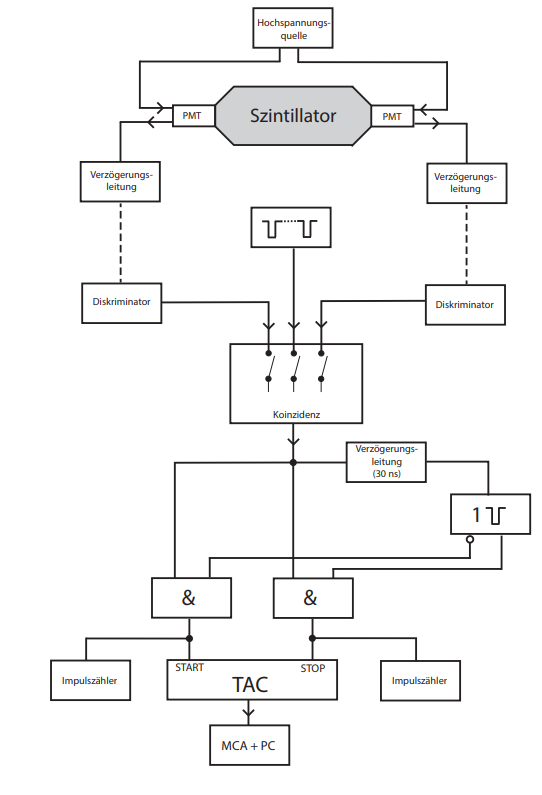
\includegraphics[scale=0.5]{fig/aufbau.png}
	\caption{Blockschaltbild des Versuchaufbaus \cite[3]{Anleitung}.}
	\label{fig:aufbau}
\end{figure}
\FloatBarrier
\noindent Im Szintillator treffen die Myonen ein und werden dort, wie in Abschnitt \ref{sec:Detektion} beschrieben, detektiert. Der Szintillator, der verwendet wird, ist organisch, da eine
geringe Abklingzeit in diesem Versuch benötigt wird und die Energieauflösung vernachlässigbar ist. \\
Die Photomultiplier (PM) an den Ausgängen des Szintillators sind für die Umwandlung der Lichtimpulse in elektrische Impulse zuständig. Die daraufhin folgende Koinzidenzschaltung ist deswegen
eingebaut, da die PMs zur spontanen Emission neigen und somit Ursache von Messfehlern sein können. Die Koinzidenzschaltung sorgt dafür, dass nur bei nahezu gleichzeitiger Impulsaussendung in
einem kleinen Intervall der beiden PMs das Signal weitergeleitet wird. Die Verzögerungsleitungen werden so angepasst, dass die Signale aus beiden PMs zeitgleich an der Koinzidenz ankommen.
Die Diskriminatoren, die ebenfalls zwischen Koinzidenzschaltung und PMs verbaut sind, sorgen für Rauschunterdrückung. \\
Die Lebensdauer der Myonen wird mit einer elektronischen Stoppuhr gemessen, die startet sobald ein Myon in den Szintillator eintritt und den Startimpuls auslöst und stoppt wenn das Myon zerfällt.
Dies wird technisch mit einem Time-Amplitude-Converter (TAC) realisiert, der einen Spannungsimpuls ausgibt, dessen Amplitude proportional zur Zeitdifferenz ist. Als letztes werden die
Spannungsimpulse des TAC von einem Multichannel-Analyzer (MCA) histogrammiert. Um diesen MCA zu kalibrieren werden mittels eines Doppelimpulsgenerators die Kanäle auf eine Zeitachse skaliert. \\
\subsection{Störeffekte}
\label{sec:Störeffekte}
Zusätzlich zu den Störeffekten durch die MPs, die durch die Koinzidenzschaltung verhindert werden sollen, existiert ein weiteres Problem. Die meisten Myonen besitzen eine zu hohe Energie
und liefern daher keinen Zerfallsimpuls. Damit keine Messfehler entstehen ist eine Logikschaltung zwischen Koinzidenz und MCA verbaut (s. Abbildung \ref{fig:aufbau}). Diese besteht aus zwei
AND-Gattern, einem Univibrator und einer Verzögerungsleitung von etwa $t_\mathrm{VZ}=\SI{30}{\nano\second}$. Ziel dieser Schaltung ist es, dass nach einer einstellbaren Suchzeit $t_\mathrm{s}$ die Gesamtschaltung in den Ausgangszustand versetzt wird. Damit soll gewährleistet werden, dass ein neuer Startimpuls aufgenommen werden kann. \\
Zu Beginn der Messung liegt am invertierten Ausgang des Univibrator ein H-Signal an, dass es dem Signal der Koinzidenzschaltung ermöglicht, das erste AND-Gatter zu nutzen und somit die Zeitmessung
des TAC beginnen zu lassen. Die Suchzeit $t_\mathrm{s}$ wird gestartet sobald, dass Signal der Koinzidenzschaltung die Verzögerungsleitung überwunden hat und am Univibrator ankommt. Dann liegt
am nicht invertierten Ausgang des Univibrator ein H-Signal an, sodass nur noch das zweite AND-Gatter vom Singal der Koinzidenzschaltung passiert werden kann. Dadurch kommt das Stoppsignal beim TAC
an und die Messung ist beendet. Trifft allerdings während der Suchzeit kein Signal am TAC ein, wird der Univibrator in seinen Ausgangszustand zurückversetzt und die Schaltung ist wieder bereit ein
neues Startsignal aufzunehmen. \\
Trotz der Elimination diverser Fehlerquellen ist dennoch ein Untergrundsignal übrig, da es möglich ist, dass innerhalb der Suchzeit ein weiteres Myon in den Szintillator eintritt.
Die Zeitdifferenz der beiden Eintritte wird dann als Lebensdauer gemessen und verfälscht die Messung, da die Myonen nicht zerfallen sind. Dieser Untergrund wird später in der Auswertung
berücksichtigt und wird durch zwei verschiedene Methoden bestimmt.
\subsection{Durchführung}
Als erstes werden die Bauteile wie in Abbildung (\ref{fig:aufbau}) verkabelt bis zu Koinzidenzschaltung verkabelt. Weiter werden nun verschiedene Verzögerungszeiten eingestellt, bei drei verschiedenen Pulsbreiten von $t_1=\SI{20}{\nano\second}$, $t_2=\SI{15}{\nano\second}$ und $t_3=\SI{10}{\nano\second}$. Nun wird die Suchzeit $t_\mathrm{s}$ eingestellt, dazu wird ein Oszilloskop an den Univibrator angeschlossen. Die gewählte Suchzeit beträgt $t=\SI{10}{\nano\second}$. \\
Im zweiten Teil wird jetzt die restliche Schaltung bis zum TCA aufgebaut und überprüft. Statt den PMs wird ein Doppelimpulsgenerator an die Koinzidenzschaltung angeschlossen, der Messbereich des TAC wird an die Suchzeit angepasst und der MCA wird angeschlossen. Um den MCA zu kalibrieren werden vom Doppelimpulsgenerator Impulse mit verschieden Zeitdifferenz erzeugt. Es wird überprüft bei welchen
Zeiten welche Kanäle gefüllt werden. Daraus wird später in der Auswertung eine Ausgleichsgerade berechnet, die den Zusammenhang zwischen Kanalnummer und Zeit beschreibt. \\
Die eigentliche Messung zur Bestimmung der Lebensdauer der kosmischen Myonen kann nun beginnen. Dabei werden über $t_\mathrm{Messung}=\SI{272190}{\second}$ Impulse aufgenommen.
